\section{Data-Driven Decision Making in Plant Care}

After the measurement cycle described in Section 2.3, Plant Up! receives structured sensor data at the backend: timestamped values for moisture, climate, and light. This chapter explains how those incoming values are interpreted and transformed into feedback that a user can act on without needing to read raw numbers.

\subsection{Threshold Zones and Plant-Specific Ranges}

Building on the safe corridors defined in Section 2.2, each incoming sensor value is compared against an ideal range stored as a plant-specific configuration. The system classifies every parameter into three condition zones: Green (optimal, no action), Yellow (close to a boundary, attention recommended), and Red (outside the safe range, action required).

This applies to soil moisture, temperature, humidity, light, and, if available, the EC of the nutrient solution. The traffic-light mapping is intentionally chosen because green, amber, and red are widely recognized as low, medium, and high status codes in everyday decision aids.

Plant-specific ranges are not a universal default. A cactus is typically configured with lower moisture tolerance and higher light tolerance, while a fern prefers higher humidity and lower exposure to direct sunlight. In Plant Up!, these differences are handled as configurable parameters per plant profile rather than hardcoded constants.

Seasonal adjustment is implemented by storing separate summer and winter ranges. The reasoning is practical: indoor climate and light availability shift with seasons, and the same plant often needs different watering frequency and different tolerance bands depending on these conditions. Instead of forcing users to retune thresholds manually, Plant Up! switches between two predefined sets while keeping them editable.

\noindent
\begin{minipage}[t]{0.55\textwidth}
    \vspace{0pt}
    To avoid overwhelming users with five separate decisions, Plant Up! computes a health score from 0\,--\,100\,\% as a combined indicator. Such composite scoring simplifies interpretation without discarding the underlying data from individual sensors. \cite{boniecki2023smartSensors} The health score compresses complexity into one overall status that is easy to scan. It is mapped to four labels: Great ($\geq$70\,\%), Okay (40\,--\,70\,\%), Needs Care (20\,--\,40\,\%), and Critical ($<$20\,\%).

    \vspace{1em}
    As shown in Figure~\ref{fig:live_data_health}, the interface exposes both layers at once: the overall health score for quick orientation and the individual sensor values for users who want to verify the cause of a warning. The Daily Mentor feature is an AI-supported component that generates short natural-language hints based on the current zone states, turning combinations like ``too dry'' and ``high temperature'' into a concrete watering suggestion.
\end{minipage}\hfill
\begin{minipage}[t]{0.4\textwidth}
    \vspace{0pt}
    \centering
    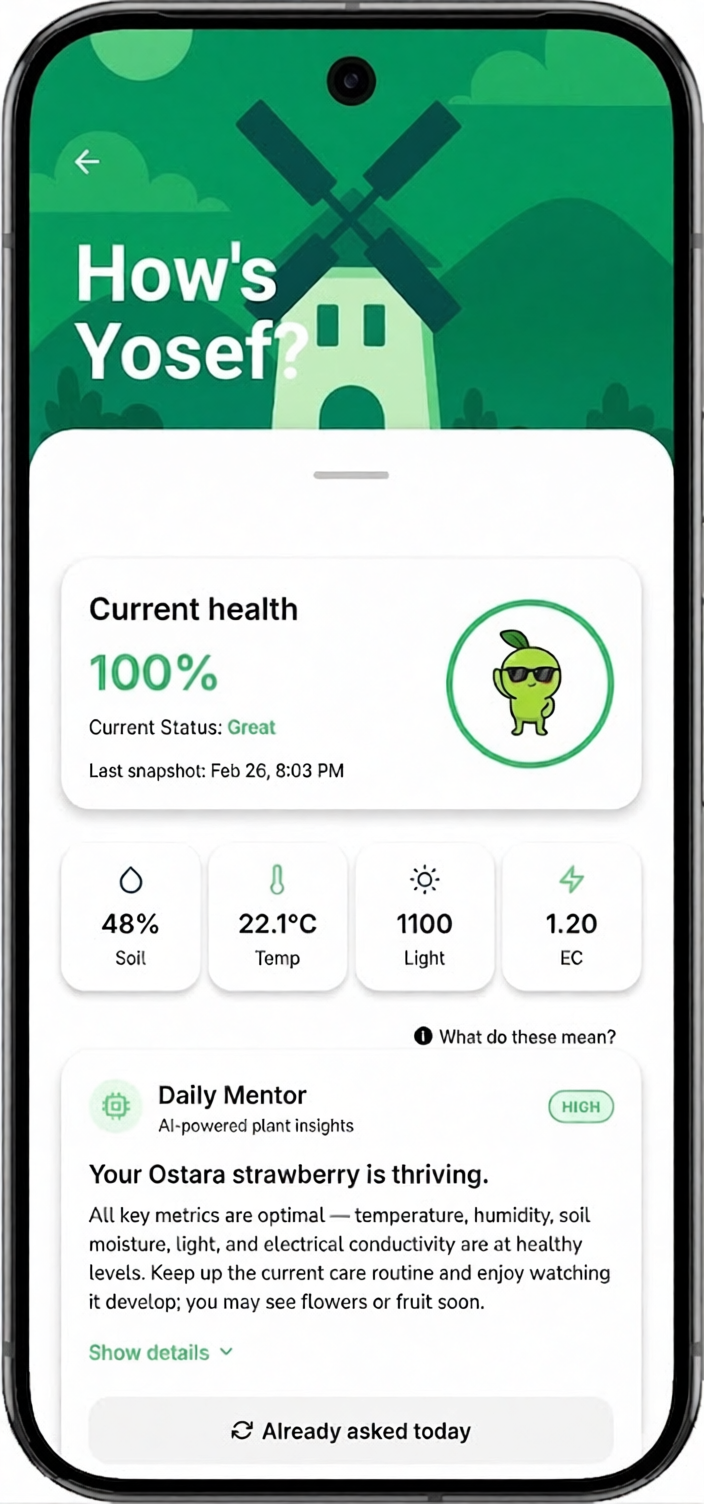
\includegraphics[width=0.8\linewidth]{images/LiveDataHealth.png}
    \captionof{figure}{Plant status overview in the Plant Up! application showing health score, individual sensor values, and AI-generated care recommendations.}
    \label{fig:live_data_health}
\end{minipage}

\vspace{1em}

\subsection{Deriving Care Recommendations}

When a value leaves its ideal range, Plant Up! generates a recommendation phrased as an action, not as a measurement. Translating raw sensor readings into specific, user-facing actions is a well-established approach in threshold-based decision support systems. \cite{dssPlantProtection} The goal is that a user reads ``Water it now'' instead of interpreting ``Soil moisture: 18\,\%'' under time pressure. The system evaluates parameters individually, and the first parameter that triggers a Yellow or Red state becomes the active recommendation until the next measurement cycle updates the situation.

\begin{figure}[H]
    \centering
    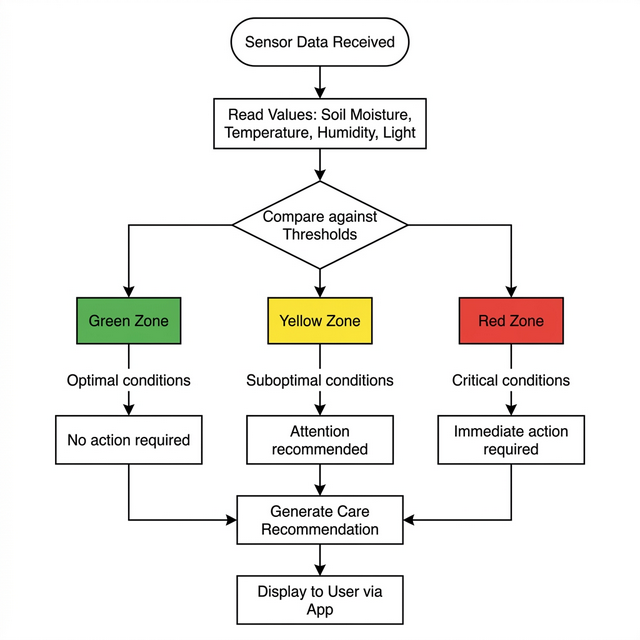
\includegraphics[width=0.7\textwidth]{images/decision_flowchart.png}
    \caption[Decision flow from sensor data to care recommendation (generated with ChatGPT 5.4, OpenAI).]{Simplified decision flow: sensor data is compared against plant-specific thresholds and classified into condition zones, which then trigger the corresponding care recommendation (generated with ChatGPT 5.4, OpenAI).}
    \label{fig:decision_flowchart}
\end{figure}

Figure~\ref{fig:decision_flowchart} summarizes this logic visually: incoming measurements are checked against stored thresholds, classified into zones, and then translated into one user-facing recommendation.

\subsection{Visualization and Interpretation}

Interpretation is not only logic. It is also presentation. Plant Up! uses a traffic-light visualization with color-coded indicators (green, yellow, red) and an animated mascot (``Sprig'') that mirrors the current plant state. The purpose is speed: users should recognize ``all good'' versus ``act now'' in one glance, even without understanding the sensor units. Using color as a semantic status channel follows the principle that red signals danger, yellow signals caution, and green signals a safe condition, a convention standardized in ISO~3864. \cite{iso3864}

\begin{figure}[H]
    \centering
    \begin{minipage}{0.3\textwidth}
        \centering
        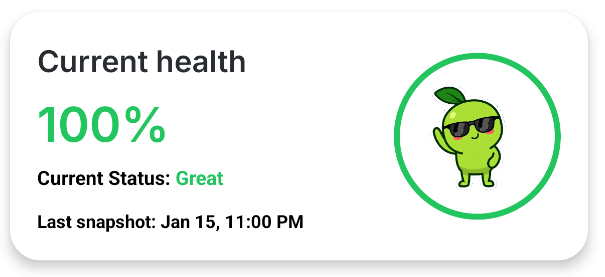
\includegraphics[width=\linewidth]{images/GreatHealth.png}
    \end{minipage}\hfill
    \begin{minipage}{0.3\textwidth}
        \centering
        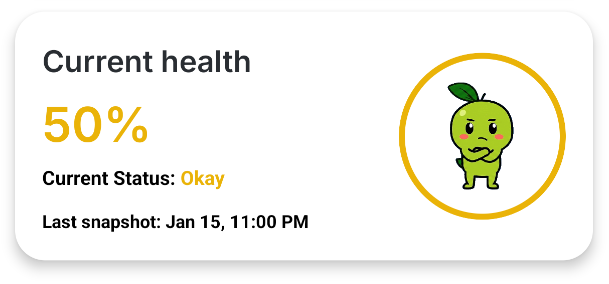
\includegraphics[width=\linewidth]{images/OkayHealth.png}
    \end{minipage}\hfill
    \begin{minipage}{0.3\textwidth}
        \centering
        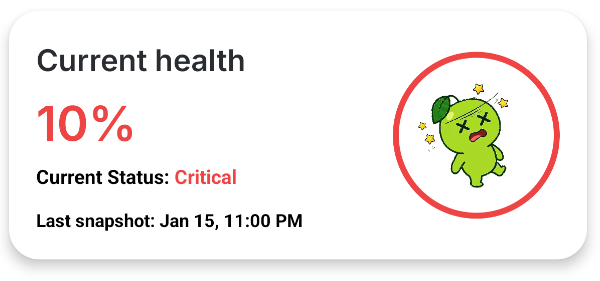
\includegraphics[width=\linewidth]{images/CriticalHealth.png}
    \end{minipage}
    \caption{Traffic light health status in Plant Up!: optimal conditions (left, 100\,\%), suboptimal conditions requiring attention (center, 50\,\%), and critical state requiring immediate action (right, 10\,\%).}
    \label{fig:health_traffic_light}
\end{figure}

Figure~\ref{fig:health_traffic_light} illustrates these three primary health states. Rather than focusing on numbers, the interface leverages the mascot's expression and the background color to immediately communicate whether the plant is thriving, needs attention, or requires urgent care.

\noindent
\begin{minipage}[t]{0.55\textwidth}
    \vspace{0pt}
    Single values are useful, but trends are where the ``why'' becomes visible. Plant Up! therefore shows historical data as bar charts with selectable time ranges (1 hour, 24 hours, 7 days, all time). Time-oriented visualizations make it easier to detect patterns and anomalies than isolated snapshots, because humans can quickly see slopes, cycles, and sudden jumps across a timeline. \cite{jmirTimeSeries}

    \vspace{1em}
    As illustrated in Figure~\ref{fig:trend_chart}, a 1-hour chart focuses on immediate short-term variations, providing live insight into sudden environmental shifts. These patterns support quick reactions and help users confirm if their immediate physical actions, like watering the plant, register correctly within the system.

    \vspace{1em}
    With these decision rules and visual mappings defined, Plant Up! can transform raw measurements into consistent feedback. The next chapter describes how this interpretation layer is implemented in the real system and tested under practical conditions.
\end{minipage}\hfill
\begin{minipage}[t]{0.4\textwidth}
    \vspace{0pt}
    \centering
    \includegraphics[width=0.9\linewidth]{images/1hourgraph.png}
    \captionof{figure}{Historical sensor data visualization in Plant Up! showing soil moisture readings over a 1-hour period. Users can switch time ranges to identify trends and patterns.}
    \label{fig:trend_chart}
\end{minipage}

\vspace{1em}
